\section*{Classification}
For any class, estimate the probability of being in such class: $\pi_j(x) = \mathbb{P}(Y = j\mid X=x)$
\textbf{Bayes estimator} is $\mathcal{C}(x) = \arg\max_j\pi_j(x)$.\\
%\textbf{KNN:} Take the $K$ nearest neighbours and have them vote, $K$ big = bias, $K$ small = variance.
%\begin{codebox}{r}{KNN}
%library(FNN)
%pred.knn <- knn.reg(train = matrix(dtrain[,1],ncol=1), test=matrix(dtest[,1], ncol=1), y = ytrain, k=i)
%  results.knn[i] <- mean((ytest - pred.knn$pred)^2
%fit <- glm(y ~ x, family = binomial, data = heart)
%\end{codebox}
\textbf{Linear discriminant analysis:} 
Assumption: $X\mid Y = j \sim \mathcal{N}(\mu_j,\Sigma)$. Prediction: $\text{arg max}_j \left( x - \frac{\hat{\mu}_j}{2}\right)^{\top} \hat{\Sigma}^{-1}\hat{\mu}_j + \text{log}(\hat{p}_j)$ Decision Boundary: B \; := \; \{x \in \mathbb{R}^d \; | \; x^{\top}\Sigma^{-1}(\mu_0 - \mu_1) = \text{log}\left( \frac{p_1}{p_0} \right) + \frac{1}{2} \mu_0^{\top} \Sigma^{-1} \mu_0 - \frac{1}{2} \mu_1^{\top} \Sigma^{-1} \mu_1\}

\textbf{QDA:} ($(J-1)p(p+1)/2$ more params) $\Sigma_j$ group-wise by looking at elements in the group and by correcting with $\frac{1}{n_j-1}$ instead of $\frac{1}{n-j}$.

$\arg\max \log\hat p_j-\log(\det\hat \Sigma_j)/2-(x-\hat \mu_j)^{\top}\hat\Sigma_j^{-1}(x-\hat\mu_j)/2$

\begin{codebox}{r}{Linear \& Quadratic Discriminant analysis}
library(MASS)
c_lda<-lda(x=data[,c("x1","x2")],grouping=data[,"y"])
c_qda<-qda(x=data[,c("x1","x2")],grouping=data[,"y"])
# Pred. performance assessment, adjust FP, FN penalty
\end{codebox}
\textbf{Logistic regression:} Let $\pi(x) = \mathbb{P}(Y=1\mid X = x)$. Estimate with a linear model $g(x) = \text{logit}(\pi(x)) = \log\frac{\pi(x)}{1-\pi(x)}$. Assuming $g(x) = X\beta$, for the log-likelyhood:
$\ell(\beta;Y,X)=\sum_{i=1}^n\left(Y_i \beta^Tx_i - \log\left(e^{\beta^Tx_i} +1\right)\right)$\\
E.g. gradient descent for minimization\\
\begin{codebox}{r}{Logistic regression}
mod <- glm(y ~ ., data = data, family = "binomial")
mod <- glm(cbind(N, m - N) ~ age, family = binomial, data = heart) # for binomial distribution. No. successes in first column!
#family="binomial" is what makes a logistic reg.
p = predict(mod, type = "response") # prob of being 1
mean((p > 0.5) == y)
# for multinomial regression #library(nnet)
class_multinom <- multinom(y ~ . , data = data)
\end{codebox}
\textbf{Comment}: LDA is a logistic regression model, since log-odds ratio is linear. But not every logistic regression model is LDA due to normal feature assumption in LDA.\\
\textbf{Techniques for multi-class:}\\
\underline{1) One versus rest}: Train a model per class against all other classes to receive $\pi_j(x)$. Normalization needed. 
\underline{2) Everyone versus reference}: Train all other $J-1$ classes against reference class $0$: $g(x) = \log(\pi_j(x)/\pi_0(x))$\\
\underline{3) Multinomial Distribution}: binomial $\rightarrow$ multinomial distr\\
\underline{4) One vs. one}
Train a model to distinguish each class from each other. In total $\binom{J}{2}$ models.\\
\underline{5) Ordered classes}: $\text{logit}(\mathbb{P}(Y\leq k \mid x))=\alpha_k +g(x)$ with $\alpha_0\leq\alpha_1\leq\dots\leq \alpha_{J-1}$ "prop. odds m." \texttt{ polr} from \texttt{MASS}\\
\textbf{ROC (Receiver Operating Characteristic):}\\
Predict $\hat Y(x) = \mathbb{I}(\hat{\pi}(x)\geq \theta)$. \\

$\text{sensitivity} = TPR = \frac{TP}{P}=\frac{TP}{TP+FN}$; estimates $\mathbb{P}(\hat{Y} = 1| Y = 1)$

$\text{specitivity} = TNR = \frac{TN}{N}$; estimates $\mathbb{P}(\hat{Y} = 0| Y = 0)$\\

Change $\theta \in [0, 1]$ to plot $TPR=f(FPR)=f(1-TNR),\; f'\geq 0$.
$\int\text{ROC}=\text{ROC AUC} = \mathbb{P}(\hat{\pi}_{I_0} < \hat{\pi}_{I_1})$, where $I_0$ and $I_1$ are sampled uniformly at random from indexes with classes $Y=0$ and $Y=1$, respectively.\\

$\text{cost} = \text{missclass. rate} = \frac{FP + FN}{TP + FP + TN + FN}$; $FPR = \frac{FP}{FP + TN}$ \\
Compute cost from TPR \& FPR \& PR:

$\text{cost} = PR \cdot (1 - TPR) + (1 - PR) \cdot FPR$
\begin{codebox}{r}{Evaluation}
#l is a vector of 0/1 (the truth)
#p is a vector of predicted probs to be 1
pred <- prediction(predictions = p, labels = l)
perf <- performance( pred, "tpr", "fpr" )
plot(perf)# plots the ROC curve
perf.c <- performance(pred, "cost", cost.fp = 1, cost.fn = 2)
plot(perf.cost)
#plots the cost changing the cutoff (cost.fp and cost.fn can be setted to have an asym loss)
#to add cross-validation
all.y.true <- all.y.pred <- vector("list", length=K)
#and we fill them with CV, then to make average ROC:
pred.cv <- prediction(all.y.pred, all.y.true)
perf.cv <- performance(pred.cv, "tpr", "fpr" )
plot(perf.cv, avg = "threshold")
plot(perf, col = 2, add = TRUE)
\end{codebox}
%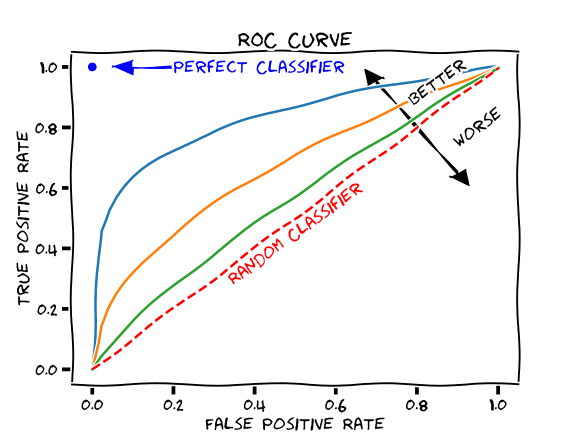
\includegraphics[width = 5cm]{ROC.png}\\